\documentclass{article}
\usepackage[utf8]{inputenc}
\usepackage[dvipdfmx]{hyperref}
\usepackage{fancyhdr}
\usepackage{caption, floatrow}

\usepackage[dvipdfmx]{graphicx}

\usepackage{mathtools}
\renewcommand{\theequation}{eq. \arabic{equation}}


\usepackage[
  style=numeric,
  citestyle=numeric,
  url=true,
  doi=false,
  isbn=false
  ]{biblatex}
\addbibresource{main.bib}


\DeclareNewFloatType{graph}{placement=H, name=Graph}
\floatsetup[graph]{capposition=bottom}


% contents below
% ------------------------------------------------------------------------------

\pagestyle{fancy}
\fancyhf{}
\rhead{Rikuo Hasegawa}
\chead{UPCSE PHYSICS Long Lab Report}
\lhead{\today}
\rfoot{p. \thepage}

\title{Measurement of the Wavelength of a Helium-neon Laser via Interference Patterns in a Reflection Grating Experiment}
\author{ Rikuo Hasegawa \\ Tutorial Group: C \\ Lab Pair: Mohammed Alsaleh }

\begin{document}

\maketitle
\thispagestyle{fancy}
\vspace*{\fill}
\parbox{\linewidth}{\centering%
Date of Experiment: January 16, 2019
\\ Date of Report Submission: January 30, 2019
\\ University Preparatory Certificate for Science and Engineering
}
\newpage

\section*{Abstract}
\paragraph{}
The aim of this experiment was to confirm the theory behind interference as light reflects off of a reflection grating and measure the wavelength of a Helium-neon (HeNe) laser. The experiment properly confirmed that our theory properly models the observed phenomenon by comparing the measured wavelength with the known wavelength of a HeNe laser, 632.8 nm \autocite{WikiHeNe}. The wavelength measured by the experiment was

$$
xxx.xx \pm \Delta xx [nm]
$$

In this report, we first introduce the theory of light interference patterns from a reflection grating. Then, we introduce the apparatus used and explain the experiment protocol. This is followed by an analysis of our results. Finally, we will discuss the results and give our conclusion.

\section{Introduction}

\subsection{Theory}
\paragraph{}
A coherent light source is a light source in which the light waves from the source are in phase. When light from a coherent light source travels through two separate paths to reach a single point in space, they undergo a phenomenon called interference. This interference can be constructive or destructive. The intensity of light at a point where constructive interference is occuring is the sum of each constructively interfering waves' intensity. On the contrary, the intensity of light due to destructive interference is 0 because in destructive interference, two waves are out of phase and cancel out. The conditions for constructive interference can be expressed as:
\begin{equation}\label{eq:constructive}
  |p_1 - p_2| = n \lambda
\end{equation}
where $|p_1 - p_2|$ is the difference between the length of the two paths that the light takes, $n$ is some natural number, and $\lambda$ is the wavelength of the light.

In this experiment, the light is reflected off a specular steel ruler with small diffuse divisions which do not reflect light onto a screen perpendicular to the ruler as seen in Figure \ref{fig:setup}. Each division of the ruler acts as a point source of light, creating an interference pattern on the screen.
\begin{figure}[H]
  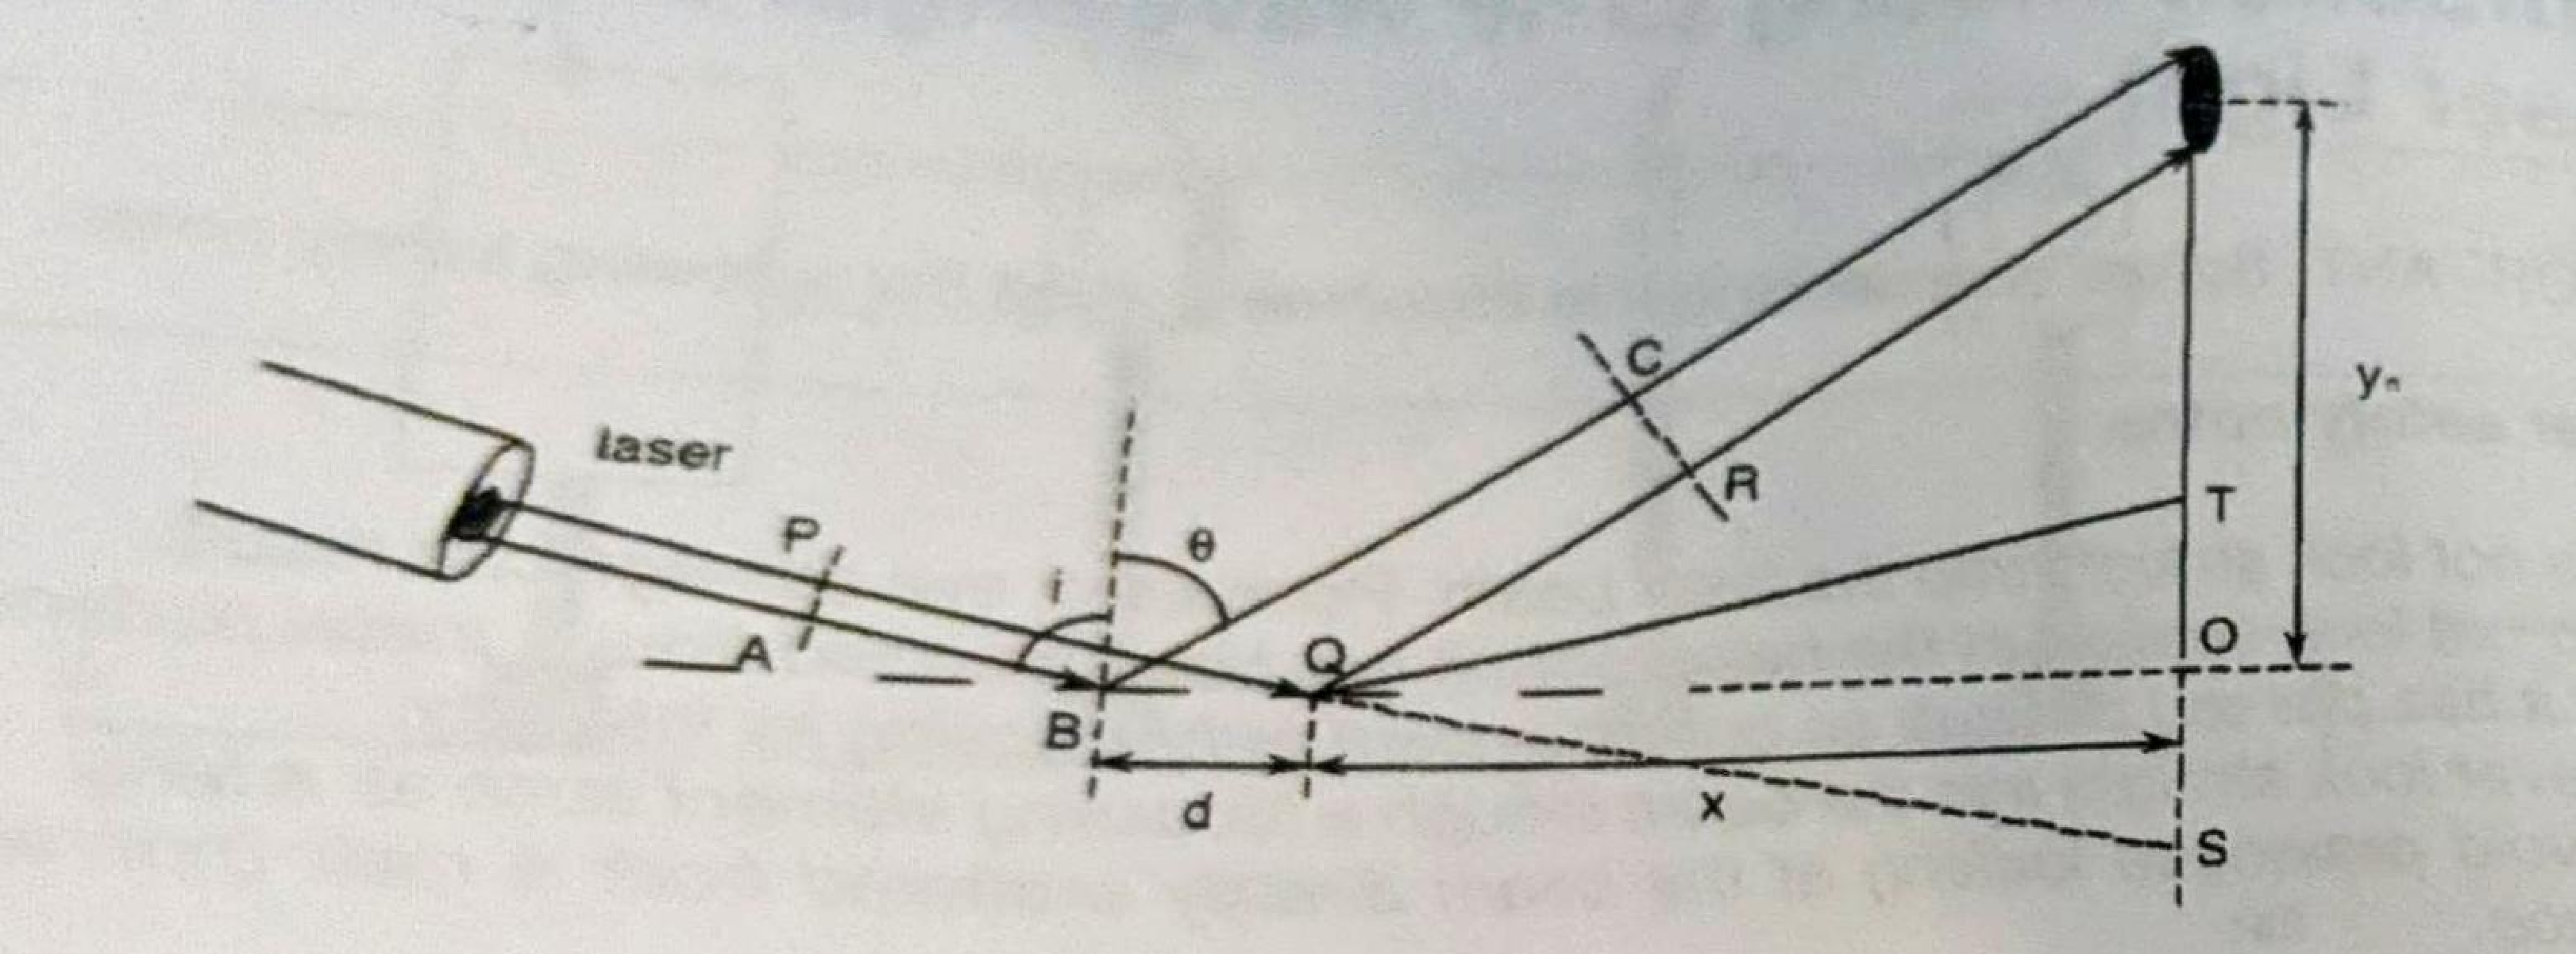
\includegraphics[width=\textwidth]{img/setup.pdf}
  \caption{The experimental setup \autocite{UPCSE2018}}
  \label{fig:setup}
\end{figure}

In Figure \ref{fig:setup}, each division is spaced by some length $d$. $x$ is the distance from the point where the laser hits the ruler to the screen where we observe the interference pattern. Point $T$ on the diagram is the point where light from pure reflection hits the screen, which also happens to be where the 0th-order peak of the interference pattern shows up. Point $S$ is where the laser would hit the screen if the ruler was not present. Thus, point $O$, the midpoint of $S$ and $T$, is also the height of the ruler projected onto the screen. When we consider the path difference of light waves that are emitted from two consecutive divisions ($PQR$ and $ABC$) as it reaches point $R$ and $C$ respectively, we can express it as in \eqref{eq:path_difference}. We measure the height of each peak of the interference pattern as $y_n$ indicating which order it is. Thus, $|OT|$ is also $y_0$.
\begin{equation}\label{eq:path_difference}
  |PQR - ABC| = d(\sin{i}-\sin{\theta})
\end{equation}

Now, recalling \eqref{eq:constructive} and \eqref{eq:path_difference}, whenever there is constructive interference, we can say that the conditions in \eqref{eq:constructive_path} are satisfied.
\begin{equation}\label{eq:constructive_path}
  n\lambda = d(\sin{i} - \sin{\theta})
\end{equation}
From Figure \ref{fig:setup} we can see:

\begin{equation}\label{eq:sin_t}
  \sin{\theta_n} = \cfrac{x}{\sqrt{x^2 + y_{n}^{2}}}
  = \cfrac{1}{
      \sqrt{1 + \left( \cfrac{y_n}{x} \right)^2}
    }
\end{equation}
Looking at the Mclaurin expansion in \eqref{eq:mclaurin} we can see that \eqref{eq:sin_t} approximates to \eqref{eq:sin_height}

\begin{equation}\label{eq:mclaurin}
  \frac{1}{\sqrt{1+z}} \approx 1 - \frac{1}{2}z \quad \text{(for $z\ll 1$)}
\end{equation}

\begin{equation}\label{eq:sin_height}
  \sin{\theta_n} = 1 - \cfrac{ y_{n}^{2} }{ 2x^2 } \quad \text{ (for $y_{n}^{2} \ll x$)}
\end{equation}
Because we are looking at a pure reflection, we can say that $i = \theta = \theta_0$. Thus, substituting $n=0$ in \eqref{eq:sin_height}, we get:

\begin{equation}\label{eq:sin_i}
  \sin{i} = 1 - \cfrac{ y_{0}^{2} }{ 2x^2 }
\end{equation}
By combining \eqref{eq:constructive_path}, \eqref{eq:sin_height}, and \eqref{eq:sin_i}, we get:

\begin{equation}\label{eq:main}
  \cfrac{
    y_{n}^{2} - y_{0}^{2}
  }{
    2x^2
  } d = \lambda n
\end{equation}
We will use \eqref{eq:main} to calculate our wavelength as the gradient of the line $\lambda n$.

As the value of $y_{n}^{2} - y_{0}^{2}$ is inversely proportional to the value of $d$ if we fix $x$ and $n$, we can expect the distance between peaks to be larger when the distance between divisions are smaller. Thus, we can expect to see less uncertainty in our measurement of $\lambda$ in the experiment with the smallest $d$ since we will be measuring $y_{n}^{2}$ directly.

\subsection{Aims and Objectives}
\paragraph{}
The aim of this experiment was to measure the wavelength of a HeNe laser.  By applying the measurements taken from our experiment setup to the theory, we calculated a measurement for the wavelength of our laser.

Another objective was to confirm how the size between divisions affected the precision of the measurement of the wavelength. By calculating the uncertainty in each experiment, we can conclude which setup led to the most precise results.

\section{Experimental Equipment and Method}
\subsection{Apparatus}

\paragraph{}
The experimental setup is shown in Figure \ref{fig:setup}. It consists of a HeNe laser placed at a shallow angle towards a specular ruler with diffuse divisions, placed at a specific distance from a screen perpendicular to the ruler and approximately perpendicular to the laser beam.
A sheet of paper is taped on the screen in order to measure the results.


\subsection{Protocol}

The experimental protocol is described below.

\begin{enumerate}
  \item Setup the equipment. In our experiment, we set the distance from the ruler to the screen ($x$) at $4.92 \times 10^{-1}$ [m]. We used divisions ($d$) of $5.08 \times 10^{-4}$ [m], $3.97 \times 10^{-4}$ [m], $2.54 \times 10^{-4}$ [m]. (1/50, 1/64, 1/100 inches).
  \item Main loop:
    \begin{enumerate}
      \item Locate point $S$ by moving the ruler to the side so it does not obstruct the laser beam. The point where the beam hits the paper is $S$.
      \item Locate point $T$ by moving the ruler so the laser beam strikes a completely specular section of the ruler. The point where the beam hits the paper is $T$.
      \item Locate point $O$ by moving the ruler horizontally towards the paper, making sure the height is unchanged. The height where the top of the ruler hits the paper is the height of $O$. Draw a line between $S$ and $T$ to locate $O$.
      \item Return the ruler back to the original position where $x$ was measured and shift the ruler along the plane parallel to the table so the beam hits the divisions. There should be an observable interference pattern on the paper along the line $OT$.
      \item Mark the each observed peak of the interference pattern from $y_0$ 10 times up until $y_9$.
    \end{enumerate}
  \item Repeat the previous step for the other 2 division sizes.
  \item Remove the paper from the screen and measure $y_0, y_1, ..., y_9$.
  \item Discard measurements where $\frac{y_n}{x} > 0.4$ as the condition for our approximation from \eqref{eq:sin_height} is no longer satisfied in this case.
\end{enumerate}


\section{Measurements and Results}
\paragraph{}
The raw measurements of $y_n$ are shown in Table \ref{tb:raw_data} for respective division sizes on the ruler.

\begin{table}[h]
\begin{tabular}{l|l|l|l|}
\cline{2-4}
                                  & \textbf{1/50 in. {[}m{]}} & \textbf{1/64 in. {[}m{]}} & \textbf{1/100 in. {[}m{]}} \\ \hline
\multicolumn{1}{|l|}{\textbf{y0}} & 0.048                     & 0.048                     & 0.031                      \\ \hline
\multicolumn{1}{|l|}{\textbf{y1}} & 0.053                     & 0.057                     & 0.047                      \\ \hline
\multicolumn{1}{|l|}{\textbf{y2}} & 0.059                     & 0.064                     & 0.059                      \\ \hline
\multicolumn{1}{|l|}{\textbf{y3}} & 0.064                     & 0.07                      & 0.069                      \\ \hline
\multicolumn{1}{|l|}{\textbf{y4}} & 0.069                     & 0.076                     & 0.078                      \\ \hline
\multicolumn{1}{|l|}{\textbf{y5}} & 0.074                     & 0.082                     & 0.087                      \\ \hline
\multicolumn{1}{|l|}{\textbf{y6}} & 0.078                     & 0.087                     & 0.094                      \\ \hline
\multicolumn{1}{|l|}{\textbf{y7}} & 0.082                     & 0.092                     & 0.101                      \\ \hline
\multicolumn{1}{|l|}{\textbf{y8}} & 0.086                     & 0.096                     & 0.107                      \\ \hline
\multicolumn{1}{|l|}{\textbf{y9}} & 0.09                      & 0.102                     & 0.114                      \\ \hline
\end{tabular}
\caption{Raw measurements of $y_n$ for each division size}
\label{tb:raw_data}
\end{table}

Rearranging the values in \eqref{eq:main}, we can see that given $y_{0}$, $x$, and $d$ are fixed, $y_{n}^{2}$ should be proportional with $n$.

\begin{equation}\label{eq:ysq}
  y_{n}^{2} = \frac{2x^2 \lambda}{d} n + y_{0}^{2}
\end{equation}
Thus, the wavelength can be expressed in terms of the gradient of the line of $y = y_{n}^{2}$, which we will refer to as $y'$ as seen in \eqref{eq:lambda}.
\begin{equation}\label{eq:lambda}
  \cfrac{
  d
  }{
  2x^2
  }y' = \lambda
\end{equation}
The graphs for $y = y_{n}^{2}$ for each respective division size are shown in Graph \ref{g:50}, Graph \ref{g:64}, and Graph \ref{g:100}.

\begin{graph}
  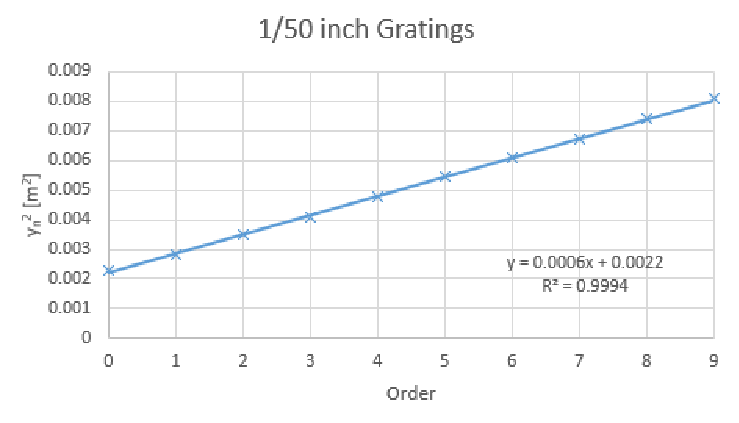
\includegraphics[width=\textwidth]{img/50.pdf}
  \caption{$y_{n}^{2}$ for each order in 1/50 in. gratings}
  \label{g:50}
\end{graph}

\begin{graph}
  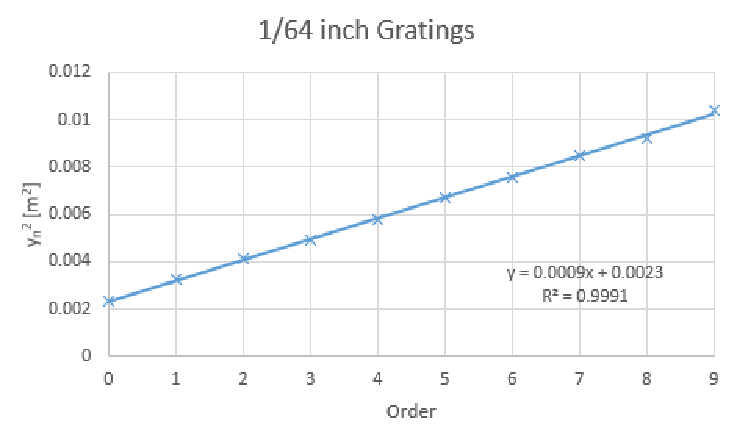
\includegraphics[width=\textwidth]{img/64.pdf}
  \caption{$y_{n}^{2}$ for each order in 1/64 in. gratings}
  \label{g:64}
\end{graph}

\begin{graph}
  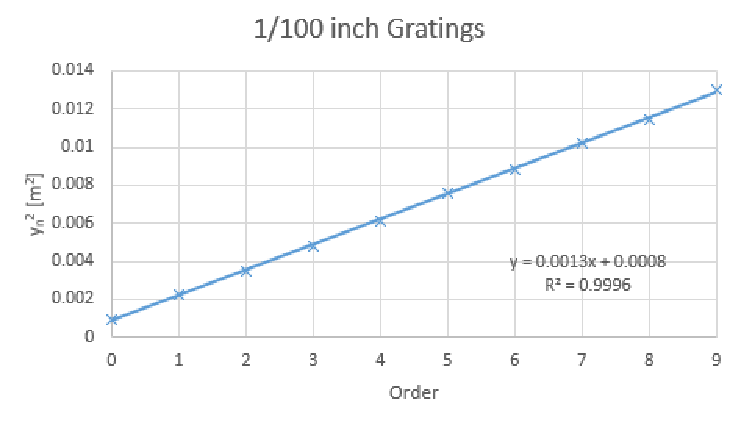
\includegraphics[width=\textwidth]{img/100.pdf}
  \caption{$y_{n}^{2}$ for each order in 1/100 in. gratings}
  \label{g:100}
\end{graph}

\section{Analysis of Results}
\paragraph{}

The graphs show the following values for $y'$:
$3.97 \times 10^{-4}$ [m], $2.54 \times 10^{-4}$

$$
\text{when}~d=\frac{1}{50}~\text{inches:}~6.00 \times 10^{-4}~[\text{m}^2]
$$
$$
\text{when}~d=\frac{1}{64}~\text{inches:}~9.00 \times 10^{-4}~[\text{m}^2]
$$
$$
\text{when}~d=\frac{1}{100}~\text{inches:}~1.30 \times 10^{-3}~[\text{m}^2]
$$
applying these values along with $d$ and $x = 4.92 \times 10^{-1}$ [m] to \eqref{eq:lambda}, the following values of $\lambda$ can be derived.
$$
\text{when}~d=\frac{1}{50}~\text{inches:}~\cfrac{5.08 \times 10^{-4} * 6.00 \times 10^{-4}}{2*(4.92 \times 10^{-1})^2} = 6.30 * 10^{-7} = \lambda
$$
$$
\text{when}~d=\frac{1}{64}~\text{inches:}~\cfrac{3.97 \times 10^{-4} * 9.00 \times 10^{-4}}{2*(4.92 \times 10^{-1})^2} = 7.38 * 10^{-7} = \lambda
$$
$$
\text{when}~d=\frac{1}{100}~\text{inches:}~\cfrac{2.54 \times 10^{-4} * 1.30 \times 10^{-3}}{2*(4.92 \times 10^{-1})^2} = 6.82 * 10^{-7} = \lambda
$$

These values are relatively close to the known true wavelength of the HeNe laser, $6.328 \times 10^{-7}$ [m]. However, this calculation does not account for the uncertainty in the measurements.

In order to calculate the uncertainty, the data is examined using the regression feature of the Microsoft Excel Data Analysis toolkit to find the upper and lower bounds for $\lambda$ within a 95\% confidence interval.

\begin{table}[H]
\begin{tabular}{|l|l|l|}
\hline
               & \textbf{Lower 95\%}    & \textbf{Upper 95\%}   \\ \hline
\textbf{1/50 in.}  & $6.68 \times 10^{-7}$ & $6.95 \times 10^{-7}$ \\ \hline
\textbf{1/64 in.}  & $7.05 \times 10^{-7}$ & $7.40 \times 10^{-7}$ \\ \hline
\textbf{1/100 in.} & $6.89 \times 10^{-7}$  & $7.12 \times 10^{-7}$ \\ \hline
\end{tabular}
\caption{Lower and upper bounds for measured wavelength within 95\% confidence interval}
\label{tb:lambda}
\end{table}

Thus, using \eqref{eq:uncertainty} \autocite{UPCSE2018} for calculating the uncertainty from the upper and lower bound of the gradient, it is possible to express the measured value with uncertainty.

\begin{equation}\label{eq:uncertainty}
  x \pm \Delta x = \frac{1}{2}(G_{upper} + G_{lower})  \pm \frac{1}{2} (G_{upper} - G_{lower})
\end{equation}

\begin{table}[H]
\begin{tabular}{|l|l|}
\hline
\textbf{division}  & \textbf{wavelength}                 \\ \hline
\textbf{1/50 in.}  & $6.82 \pm 0.135 \times 10^{-7}$ [m] \\ \hline
\textbf{1/64 in.}  & $7.23 \pm 0.175 \times 10^{-7}$ [m] \\ \hline
\textbf{1/100 in.} & $7.01 \pm 0.115 \times 10^{-7}$ [m] \\ \hline
\end{tabular}
\caption{Values of the wavelength for each division size with uncertainty}
\label{tb:result}
\end{table}

It can be seen that the uncertainty is smaller when the division size is smaller, as expected. However, the smallest systematic error is seen when the division size is the greatest.

\section{Discussion and Conclusion}
\paragraph{}
The main aim of this experiment was to measure the wavelength of the HeNe laser beam experimentally. A subtask was to decide which division size provided the most precise measurement of the wavelength.

The results are summarized in Table \ref{tb:result}.



\printbibliography
\end{document}
